\documentclass[conference]{IEEEtran}
\IEEEoverridecommandlockouts
% The preceding line is only needed to identify funding in the first footnote. If that is unneeded, please comment it out.
\usepackage{xeCJK}
\usepackage{cite}
\usepackage{amsmath,amssymb,amsfonts}
\usepackage{algorithmic}
\usepackage{graphicx}
\usepackage{textcomp}
\usepackage{xcolor}
\usepackage{subfigure}
% \usepackage{subcaption}
% \usepackage{xeCJK}
\setCJKmainfont{cwTeXKai}


\def\BibTeX{{\rm B\kern-.05em{\sc i\kern-.025em b}\kern-.08em
    T\kern-.1667em\lower.7ex\hbox{E}\kern-.125emX}}


\begin{document}

\title{Deep Learning HW2\\
% {\footnotesize \textsuperscript{*}Note: Sub-titles are not captured in Xplore and
% should not be used}
\thanks{Identify applicable funding agency here. If none, delete this.}
 
}

\author{\IEEEauthorblockN{1\textsuperscript{st} 楊淳先}
\IEEEauthorblockA{\textit{Institute of Data Science} \\
\textit{National Cheng Kung University}\\
Tainan, Taiwan \\
re61110404@gs.ncku.edu.tw}


% \and
% \IEEEauthorblockN{6\textsuperscript{th} Given Name Surname}
% \IEEEauthorblockA{\textit{dept. name of organization (of Aff.)} \\
% \textit{name of organization (of Aff.)}\\
% City, Country \\
% email address or ORCID}
}


\maketitle

\begin{abstract}
Under the previous mention of only using numpy, a two-layer neural network model and LeNet5 model were implemented, and LeNet5 was improved and compared with the original model.
\end{abstract}

\begin{IEEEkeywords}
Fully Connect Layer, Backpropagation, LeNet5
\end{IEEEkeywords}

\section{Introduction}

This assignment needs to use non-CNN-related packages such as numpy and SKLearn to implement a two-layer neural network model and LeNet-5 without using mainstream neural network packages such as Tensorflow and PyTorch.The model should calculate backward  parameters, in order to get it's gradient . In the part of LeNet5, you can refer to the github URL provided by the teacher and add your own annotations.All code can be found at \href{https://github.com/OhhhYaaa/-Deep-Learning-HW2}{https://github.com/OhhhYaaa/-Deep-Learning-HW2}.

\section{Implementation}

    \subsection{Computational Graph}
    The first question is to implement a two-layer fully connected layer, which needs to include an input layer, a hidden layer, and an output layer. As shown in the figure \ref{fig:twolayerfc}, that is to say, assuming that X is the input value, $\hat{\mathbf{y}}$ is the predicted value, $W_1$ and $W_2$ are respectively in the two layers The linear transformation matrix that needs to go through, $b_1$ and $b_2$ are the bias that need to be added in the two layers, $Sigmoid$ and $Softmax$ is the activation function used in the two-layer fully connected layer I made.
    \begin{align}
        \hat{y} = Softmax(W_2(Sigmoid(W_1 X + b_1)) + b_2)
    \end{align}

    \begin{figure}[htb]
        \centering
        \includegraphics[width=0.45\textwidth]{TwoLayerNN_adjusted.png}
        \caption{TwoLayerNN}
        \label{fig:twolayerfc}
    \end{figure}
        
    \indent In addition, during the training, the efficiency will be very poor if the gradient is updated once only one sample is viewed at a time. I hope to update multiple samples at a time, so I hope to add dataloader to help me get batch samples in each training , but since the dataloader provided in python is in PyTorch, it cannot be used, so I wrote a dataloader myself to help me iterate the samples. In addition, when calculating the loss, I use CrossEntropy for calculation. He needs to make the input matrix dimensions the same to perform the calculation, so I also wrote a onehot function to transform the label into onehot encoding.
    \indent Special mention here that I designed a activation function by myself, trying to imporve the predict accuracy.The function are shown in equation \ref{self_act}.
    \begin{align}
        0.5\cdot\left(1+\tanh\left(0.5\cdot x\right)\right)
        \label{self_act}
    \end{align}
    

    \indent The followings are the step that I calculate the gradient.First , we set some variable to represent the temporary storage used in the middle.\
    \begin{equation}
        \begin{aligned}
            z_1 &= W_1 * X + b_1 \\ 
            a_1 &= Softmax(z_1) \\
            z_2 &= W_2 * a_1 + b_2 \\
            a_2 &= Softmax(z_2)
        \end{aligned}
    \end{equation}
    
    And now let's start the backpropagation of our model:
    \begin{equation}
        \begin{aligned}
            \mathrm{d}y &= \hat{\mathbf{y}} - label \\ 
            \mathrm{d}w_2 &= \mathrm{d}a_1 * \mathrm{d}y \\ 
            \mathrm{d}b_2 &= \mathrm{d}y \\ 
            \mathrm{d}s &= \mathrm{d}w_2 * \mathrm{d}y * a_1 * (1 - a_1) \\ 
            \mathrm{d}w_1 &= X * \mathrm{d}s \\ 
            \mathrm{d}b_1 &= \mathrm{d}s
        \end{aligned}
    \end{equation}

    \subsection{LeNet-5}
    The second question is to let us implement LeNet-5. LeNet-5 is a model proposed by Professor Yann LeCun in the paper Gradient-based learning applied to document recognition in 1998. It is the first convolution successfully applied to digital recognition problems.On the MNIST dataset, the LeNet-5 model can achieve an accuracy rate of about 99.2\%.
    \indent First, let's briefly introduce the LeNet-5 model, figure \ref{fig:LeNet5_structure} shows the model structure of LeNet5, below is the seven layer of LeNet5:
    \begin{enumerate}
        \item C1 : Convolutional Layer : 
        \begin{itemize}
            \item input size : 32*32*1
            \item kernel size: 5
            \item depth : 6
            \item stride : 1
            \item padding : 0
            \item output size : 28*28*6
        \end{itemize}
        \item S2 : Pooling Layer
        \begin{itemize}
            \item input size : 28*28*6
            \item output size : 14*14*6
        \end{itemize}
        \item C3 : Convolutional Layer
        \begin{itemize}
            \item input size : 14*14*6
            \item kernel size: 5
            \item depth : 16
            \item stride : 1
            \item padding : 0
            \item output size : 10*10*16
        \end{itemize}
        \item S4 : Pooling Layer
        \begin{itemize}
            \item input size : 10*10*16
            \item output size : 5*5*16
        \end{itemize}
        \item FC5 : Fully Connected Layer
        \begin{itemize}
            \item input size : 5*5*16
            \item output size : 1*120
        \end{itemize}
        \item FC6 : Fully Connected Layer
        \begin{itemize}
            \item input size : 1*120
            \item output size : 1*84
        \end{itemize}
        \item FC7 : Fully Connected Layer
        \begin{itemize}
            \item input size : 1*84
            \item output size : 1*10
        \end{itemize}         
    \end{enumerate}

    \begin{figure}[htb]
        \centering
        \includegraphics[width=0.45\textwidth]{LeNet5_structure.png}
        \caption{LeNet5_structure}
        \label{fig:LeNet5_structure}
    \end{figure}
    
    For MNIST dataset, All pictures are after gray scale, so the input channel would be 1, but for our dataset, the input channel would be 3. And for the final output of the model, because there are 50 different labels in our dataset, instead of 10 for MNIST.So we need to modify the model to let the model train on our data.
    
    \indent First, we have to change the input size of C1, which should be changed from 32*32*1 to 32*32*3, and for the final output size, it should become 1*50. The following are the changes in the dimention of the input data. $32*32*3 \rightarrow 28*28*6 \rightarrow 14*14*6 \rightarrow 16*10*10 \rightarrow  16*5*5 \rightarrow  1*120 \rightarrow 1*84 \rightarrow 1*50$
    
    \indent By the way, the activation function in the Source code is ReLU, But in the paper, it used Sigmoid function.So, I used Sigmoid instead of ReLU in my implementation.But I find out that the backward function in Sigmoid function the source code gave is wrong.it says that the backpropagation is
    
    \begin{equation}
        \begin{aligned}
            f(x) &= \frac{1}{1 + e^{-x}} \\
            f'(x) &= x * (1 - x)
        \end{aligned}
    \end{equation}
    
    But after my calculation, I think it's backward should be 
    \begin{equation}
        \begin{aligned}
            f(x) &= \frac{1}{1 + e^{-x}} \\
            f'(x) &= \frac{1}{1 + e^{-x}} * (1 - \frac{1}{1 + e^{-x}})
        \end{aligned}
    \end{equation}
    
    \subsection{Improved LeNet-5}
    In Improved LeNet-5 model, first we have to change activation function to below
    \begin{equation}
        f(x) = x * \frac{1}{1 + e^{-x}}
    \end{equation}
    And the backpropagation should be 
    \begin{equation}
        f'(x) = \frac{1}{1 + e^{-x}} + x * \frac{1}{1 + e^{-x}} * (1 - \frac{1}{1 + e^{x}})
    \end{equation}
    And if we let $\sigma(x) = x * \frac{1}{1 + e^{-x}}$, then we can simplified above as
    \begin{equation}
        f'(x) = \sigma(x) * f(x) * \sigma(x)
    \end{equation}
    Second, we have to change the kernel size of convolutional layer from 5 to 3, and add one more convolutional layer to the model.But because it would take too much for training on 256*256 figure, I reshaped the data into 32*32.Because the figure is too small, so I take away one of the pooling layer away. So the model structure are shown in figure \ref{fig:Improved_LeNet5_structure}, which would be like
    \begin{equation}
    \begin{aligned}
        C1 &: 32*32*3 \rightarrow 30*30*6 \\
        S2 &: 30*30*6 \rightarrow 15*15*6 \\
        C3 &: 15*15*6 \rightarrow 13*13*16 \\
        padding &: 13*13*16 \rightarrow 14*14*16 \\
        S4 &: 14*14*16 \rightarrow 7*7*16 \\
        padding &: 7*7*16 \rightarrow 8*8*16 \\
        C5 &: 8*8*16 \rightarrow 6*6*6 \\
        FC6 &: 6*6*6 \rightarrow 1*120 \\
        FC7 &: 1*120 \rightarrow 1*84 \\
        FC8 &: 1*84 \rightarrow 1*50
    \end{aligned}
    \end{equation}
    \begin{figure}[htb]
        \centering
        \includegraphics[width=0.45\textwidth]{Improved_LeNet5_structure.png}
        \caption{Improved_LeNet5_structure}
        \label{fig:Improved_LeNet5_structure}
    \end{figure}
    \indent Originally, for LeNet5 and Improved LeNet5, it takes more than 2 hours to train one epoch, So I changed the forward and backward calculation of Conv and MaxPool, trying to accelarate the speed of training.Finally, it only take sixteen and twenty two minutes for one epoch, seperately.
    \indent And I discovered that the backward calculation of Conv in the source code didn't record the gradient of W and B so I plus the gradient in order to improve the result.

\section{RESULTS}
    \subsection{Computational Graph}
        Below are the results of comparing my two layer perceptron with one layer perceptron in SKLearn.For SKLearn perceptron, I trained for 2000 epochs, but for my own two layer perceptron , I only trained for 200 epochs. And figure \ref{fig:perceptron} represents the loss and accuracy while training my own two layer perceptron.\ref{fig:perceptron_self_act} represents the loss and accuracy while train two layer perceptron with my own activation function. According to the result,the curve have become gentle , so I think it can converege well and give not bad prediction.
        \begin{table}[htb]
        \begin{center}
            \begin{tabular}{l|l|l|l}
                             &   Train   &   Val  &   Test  \\ \hline
            \textbf{Mine With Sigmoid}    &   0.074  & 0.0689 & 0.0644 \\ 
            \textbf{Mine With Own Act}    &   0.2487  & 0.1533 & 0.1622  \\ 
            \textbf{SKLearn} &   0.0501  & 0.0511 & 0.0444  \\ 
        \end{tabular}
        \end{center}
        \end{table}
        

        \begin{figure}[htb]
            \centering
            \renewcommand{\figurename}{Figure}
                \subfigure[perceptron\_loss]{
                    \label{Fig:perceptron_loss}
                    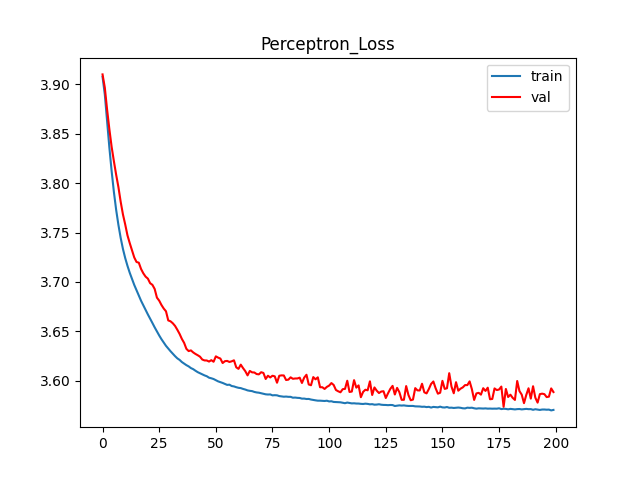
\includegraphics[width=0.2\textwidth]{perceptron_loss.png}
                }
                \subfigure[perceptron\_acc]{
                    \label{Fig:perceptron_acc}
                    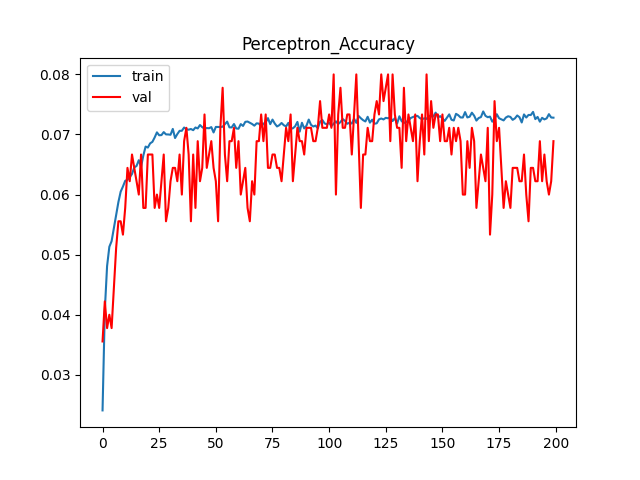
\includegraphics[width=0.2\textwidth]{perceptron_acc.png}
                }
            \caption{Perceptron\_Sigmoid}
            \label{fig:perceptron}
        \end{figure}

        \begin{figure}[htb]
            \centering
            \renewcommand{\figurename}{Figure}
                \subfigure[perceptron\_loss\_act]{
                    \label{Fig:perceptron_loss_act}
                    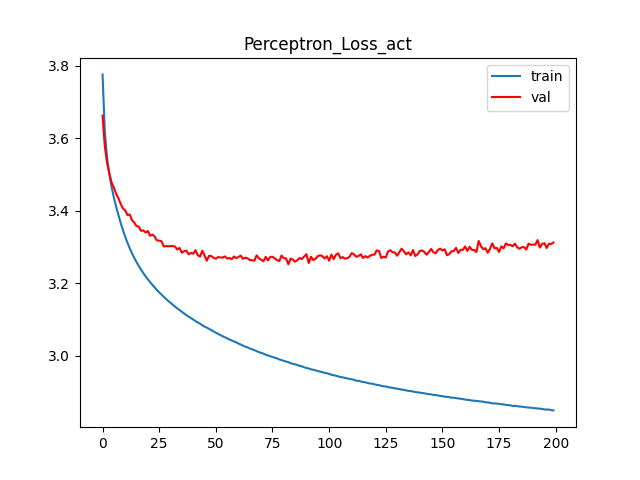
\includegraphics[width=0.2\textwidth]{perceptron_loss_act.png}
                }
                \subfigure[perceptron\_acc\_act]{
                    \label{Fig:perceptron_acc_act}
                    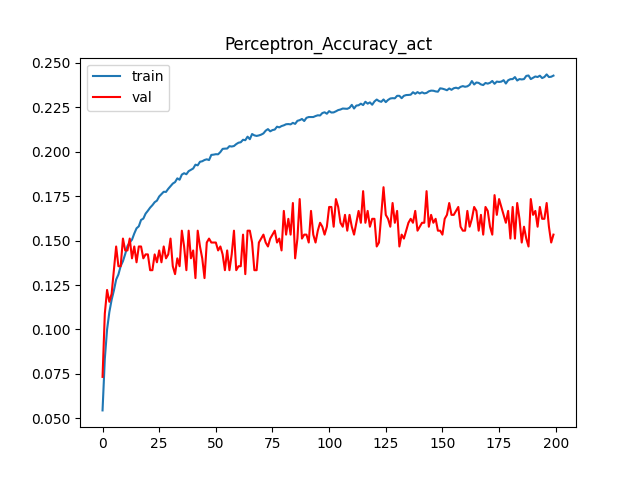
\includegraphics[width=0.2\textwidth]{perceptron_acc_act.png}
                }  
            \caption{Perceptron\_Self\_Act}
            \label{fig:perceptron_self_act}
        \end{figure}
        
    \subsection{LeNet-5}
    Below are the table comparing the original LeNet5 and Improved LeNet5.By the way I trainall of the model for 30 epochs.Figure \ref{Fig:lenet5_acc} and \ref{Fig:lenet5_loss} represent the accuracy and loss of original LeNet5 seperately.Figure \ref{Fig:Improved_lenet5_acc} and \ref{Fig:Improved_lenet5_loss} represent the accuracy and loss of Improved LeNet5 seperately.And for figure \ref{Fig:lenet5_loss_grad} and \ref{Fig:lenet5_acc_grad} represents the loss and accuracy of adding gradient of W and B.
        

    \begin{table}[htb]
    \begin{center}
        \begin{tabular}{l|l|l}
                          &   Val    &   Test     \\ \hline
        \textbf{LeNet5}   &   0.1244   &  0.1178 \\ 
        \textbf{LeNet5grad}   &   0.0956   &  0.1689 \\ 
        \textbf{Improved} &   0.0689 &  0.0978 \\ 
        \textbf{Improvedgrad} &   0.1644 &   0.1689 \\ 
    \end{tabular}
    \end{center}
    \end{table}

    \begin{figure}[htb]
        \centering
        \renewcommand{\figurename}{Figure}
            \subfigure[lenet5\_loss]{
                \label{Fig:lenet5_loss}
                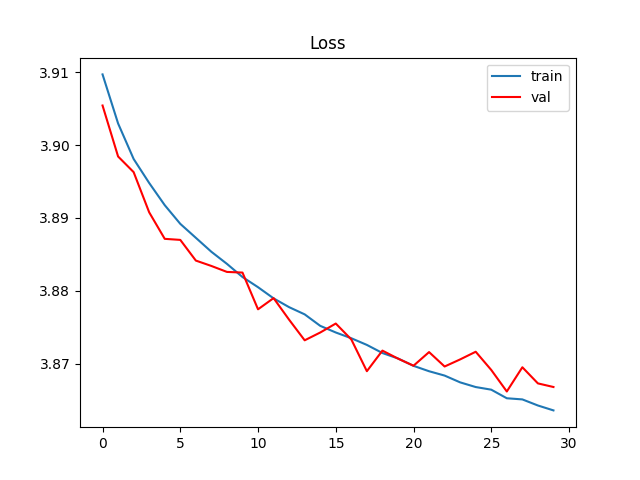
\includegraphics[width=0.2\textwidth]{lenet5_loss.png}
            }
            \subfigure[Improved\_lenet5\_loss]{
                \label{Fig:Improved_lenet5_loss}
                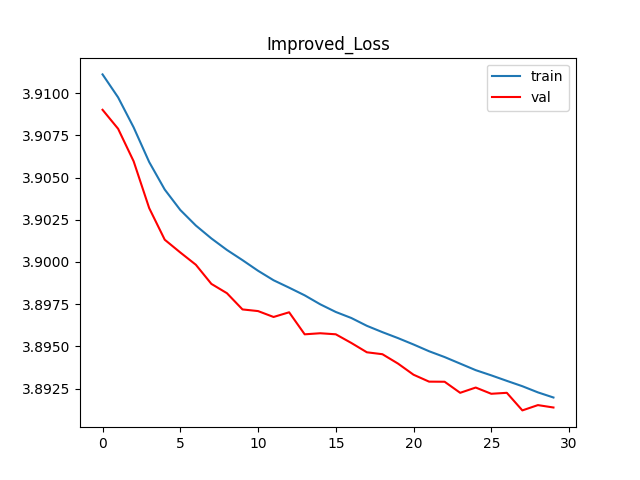
\includegraphics[width=0.2\textwidth]{Improved_lenet5_loss.png}
            }
            
        \caption{LeNet5\_Loss}
        \label{fig:loss}
    \end{figure}

    \begin{figure}[htb]
        \centering
        \renewcommand{\figurename}{Figure}
            \subfigure[lenet5\_acc]{
                \label{Fig:lenet5_acc}
                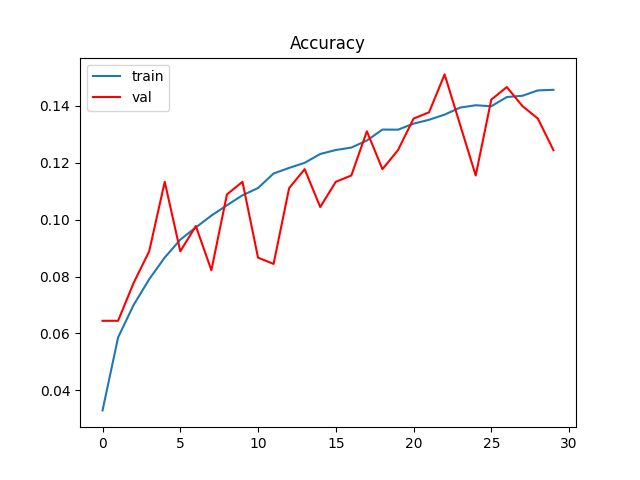
\includegraphics[width=0.2\textwidth]{lenet5_acc.png}
            }
            \subfigure[Improved\_lenet5\_acc]{
                \label{Fig:Improved_lenet5_acc}
                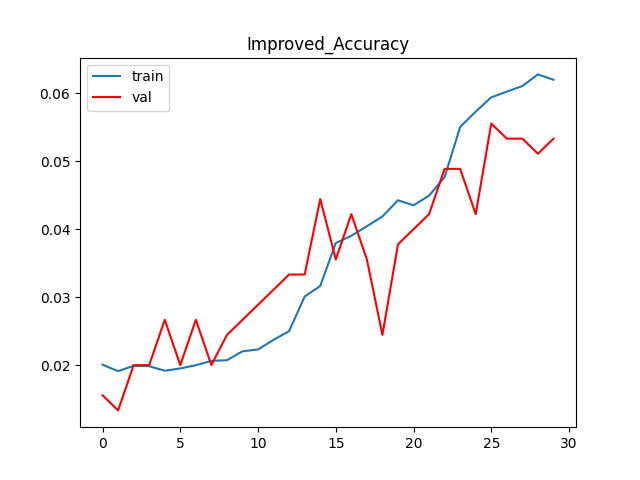
\includegraphics[width=0.2\textwidth]{Improved_lenet5_acc.png}
            }  
        \caption{LeNet5\_acc}
        \label{fig:acc}
    \end{figure}

    \begin{figure}[htb]
        \centering
        \renewcommand{\figurename}{Figure}
            \subfigure[lenet5\_loss]{
                \label{Fig:lenet5_loss_grad}
                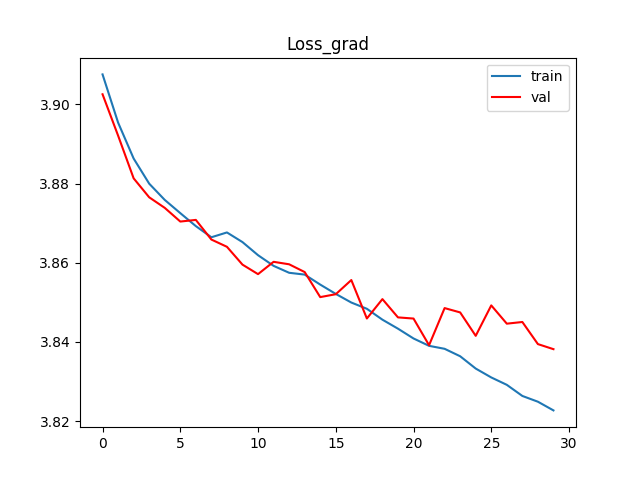
\includegraphics[width=0.2\textwidth]{lenet5_loss_grad.png}
            }
            \subfigure[Improved\_lenet5\_loss]{
                \label{Fig:Improved_lenet5_loss_grad}
                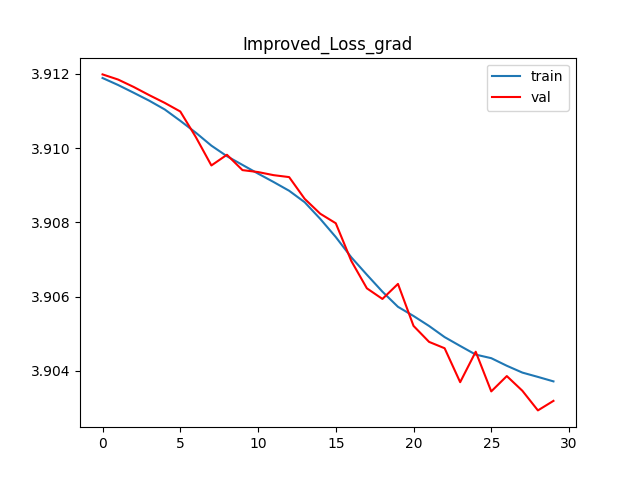
\includegraphics[width=0.2\textwidth]{Improved_lenet5_loss_grad.png}
            }
            
        \caption{LeNet5\_Loss\_grad}
        \label{fig:loss_grad}
    \end{figure}

    \begin{figure}[htb]
        \centering
        \renewcommand{\figurename}{Figure}
            \subfigure[lenet5\_acc]{
                \label{Fig:lenet5_acc_grad}
                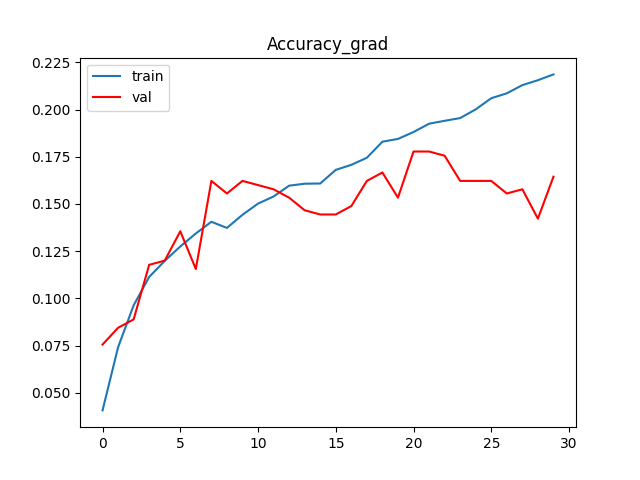
\includegraphics[width=0.2\textwidth]{lenet5_acc_grad.png}
            }
            \subfigure[Improved\_lenet5\_acc]{
                \label{Fig:Improved_lenet5_acc_grad}
                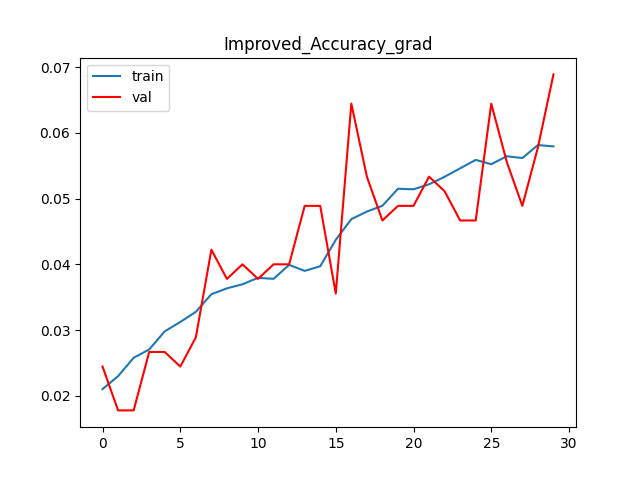
\includegraphics[width=0.2\textwidth]{Improved_lenet5_acc_grad.png}
            }  
        \caption{LeNet5\_acc\_grad}
        \label{fig:acc_grad}
    \end{figure}



        
        
\section{CONCLUSION}
It shows that my own activation would help the two layer perceptron performed better, And for LeNet5, after adding gradient of the model, the loss of the model can drop down faster.
\indent In my implementation, two layer perceptron performs the best , it can reach accuracy 24.87\%, and the worst is Improved LeNet5, which can only get 6.9\%, I guess the reason that Improved LeNet5 performs more worse than LeNet5 is because I didn;t set the depth of convolution layer well, which result in bad performance.

% \section{REFERENCE}


\begin{thebibliography}{00}
\bibitem{b1} https://github.com/toxtli/lenet-5-mnist-from-scratch-numpy
\bibitem{b2} https://chih-sheng-huang821.medium.com/\%E6\%B7\%B1\%E5\%BA\%A6\%E5\%AD\%B8\%E7\%BF\%92-weight-initialization\%E5\%92\%8Cbatch-normalization-f264c4be37f5
\bibitem{b3} https://betterprogramming.pub/how-to-build-2-layer-neural-network-from-scratch-in-python-4dd44a13ebba
\bibitem{b4} https://blog.csdn.net/Sophia\_11/article/details/85043685
\end{thebibliography}


\end{document}
